\documentclass[12pt]{article}

\usepackage{blindtext}
\usepackage{alphabeta}
\usepackage[utf8]{inputenc}
\usepackage{hyperref}

\usepackage{titling}
\usepackage{fancyvrb,minted,tcolorbox}
\usepackage{graphicx}
\graphicspath{{images/}}

\usepackage[margin=0.92in]{geometry}
\usepackage{amsmath}
\usepackage{amssymb}
\usepackage{unicode-math}
\usepackage{polyglossia}
\setdefaultlanguage{greek}
\setotherlanguage{english}
\usepackage[english=british]{csquotes}

\usepackage{xcolor}
\usepackage{amsthm}
\usepackage{thmtools}
\usepackage{svg}
\usepackage{tikz}
\usepackage{siunitx}
\usetikzlibrary{er, positioning, arrows.meta}

\tcbuselibrary{skins,breakable,breakable}
\tcbuselibrary{hooks, minted}
\usemintedstyle{monokai}

\definecolor{PastelRed}{HTML}{FAA0A0}
\definecolor{LightGray}{gray}{0.9}
\definecolor{BackgroundBlack}{RGB}{0, 0, 0}
\definecolor{BorderBlack}{RGB}{64, 64, 64}

\setromanfont{Libertinus Serif}
\setsansfont{Libertinus Sans}
\setmonofont{Liberation Mono}

\setmintedinline{fontsize=\footnotesize}

\tcbset{tcbkao/.style={
    breakable,
    before skip=\topskip,
    after skip=\topskip,
    left skip=0pt,
    right skip=0pt,
    top=5pt,
    bottom=3pt,
    left=2pt,
    right=2pt,
    sharp corners,
    boxrule=0pt,
    frame hidden,
}}

\declaretheoremstyle[
    bodyfont=\normalfont\itshape,
    headpunct={},
]{kaoplain}
\declaretheorem[
    name={Ερώτηση},
    style=kaoplain,
    numberwithin=section
]{question}
\tcolorboxenvironment{question}{
    colback=PastelRed!45!white,tcbkao
}

\renewcommand\theFancyVerbLine{\parbox{10pt}{\scriptsize\arabic{FancyVerbLine}}}

\newtcblisting{codeless}[1]{
    listing engine=minted,
    minted options app={fontsize=\footnotesize, autogobble},
    minted language=#1,
    enhanced,
    colback=BackgroundBlack,
    colframe=BorderBlack,
    listing only
}

\newcommand\ishell[1]{\codex[shell-session]{#1}}


\begin{document}

\author{
    Μπίλιας Ευστάθιος
    \\el20800
    \and
    Γκούντης Βασίλης
    \\el20636
}


\title{Μηχανισμοί Εικονικής Μνήμης}

\begin{titlepage}
    \begin{center}

        \Huge
        \textbf{Λειτουργικά Συστήματα Υπολογιστών}

        \vspace{0.5cm}
        \LARGE
        $3^η$ Εργαστηριακή Άσκηση      

        \vspace{0.3cm}
        {\vspace{-2em}\let\newpage\relax\maketitle\vspace{-2em}}

        \vspace{0.8cm}

        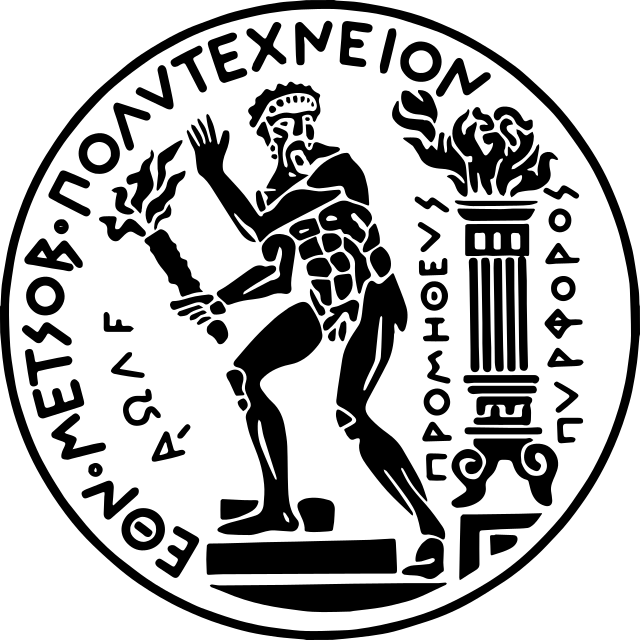
\includegraphics[width=0.3\textwidth]{logo.png}

        \vspace{0.8cm}
        \Large
        ΣΗΜΜΥ\\
        Εθνικό Μετσόβιο Πολυτεχνείο\\

    \end{center}
\end{titlepage}

\tableofcontents
\setcounter{page}{2}
\pagebreak

\section{Κλήσεις συστήματος και βασικοί μηχανισμοί του ΛΣ για τη διαχείριση της
εικονικής μνήμης}


\begin{question}
Τυπώστε το χάρτη της εικονικής μνήμης της τρέχουσας διεργασίας.
\end{question}

\begin{codeless}{c}
    /*
	 * Step 1: Print the virtual address space layout of this process.
	 */

	printf(RED "\nStep 1: Print the virtual address space map of this "
		"process [%d].\n" RESET, mypid);
	press_enter();

	/*
	 * TODO: Write your code here to complete Step 1.
	 */	

	show_maps();
\end{codeless}

\centerline{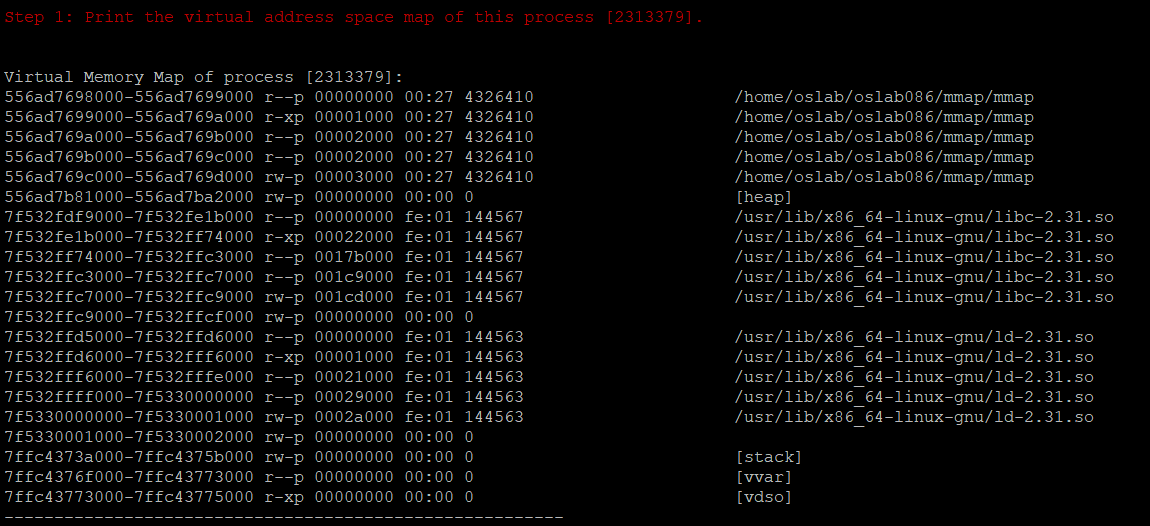
\includegraphics[width=1\textwidth]{3_1_1.png}}

\begin{question}
Με την κλήση συστήματος \textbf{mmap()} δεσμεύστε buffer (προσωρινή μνήμη) μεγέθους
μίας σελίδας (page) και τυπώστε ξανά το χάρτη. Εντοπίστε στον χάρτη μνήμης τον
χώρο εικονικών διευθύνσεων που δεσμεύσατε.
\end{question}

\begin{codeless}{c}
    /*
	 * Step 2: Use mmap to allocate a buffer of 1 page and print the map
	 * again. Store buffer in heap_private_buf.
	 */

	printf(RED "\nStep 2: Use mmap(2) to allocate a private buffer of "
		"size equal to 1 page and print the VM map again.\n" RESET);
	press_enter();

	/*
	 * TODO: Write your code here to complete Step 2.
	 */

	heap_private_buf = mmap(NULL, buffer_size, PROT_READ | PROT_WRITE, MAP_PRIVATE | MAP_ANONYMOUS, fd, 0);

   	if (heap_private_buf == MAP_FAILED) 
    {
        perror("mmap");
        exit(EXIT_FAILURE);
    }
	
    printf("Allocated memory at %p\n", heap_private_buf);

    show_maps();
\end{codeless}

Ο νέος χάρτης αφού χρησιμοποιήσαμε την mmap να δεσμεύσουμε buffer μεγέθους μιας σελίδας:

\centerline{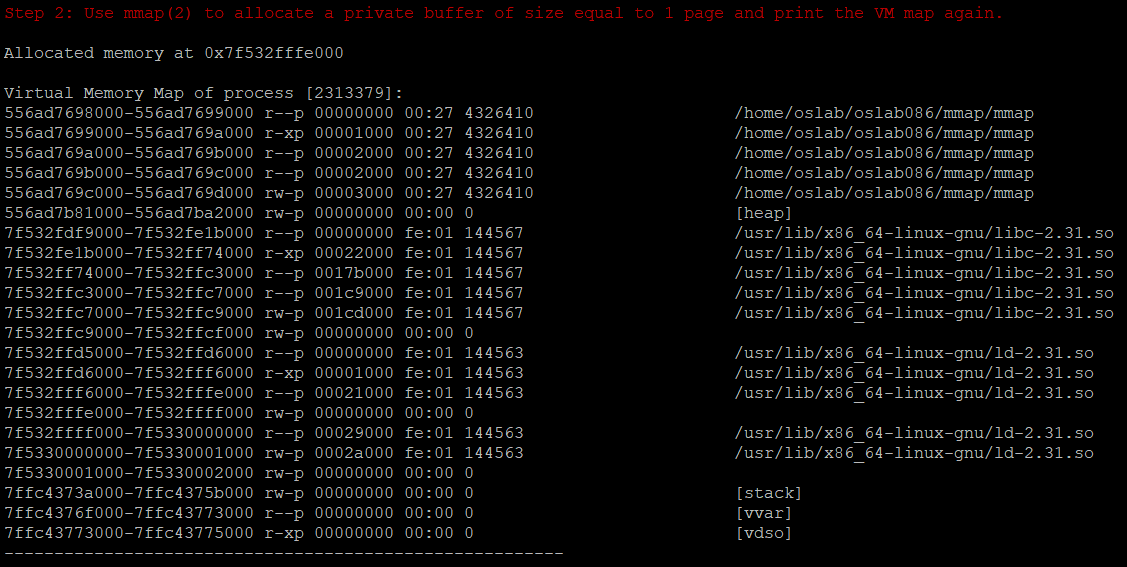
\includegraphics[width=1\textwidth]{3_1_2.png}}

Παρατηρούμε ότι αυτή η γραμμή περιέχει τον χώρο εικονικών διευθύνσεων που δεσμεύσαμε:

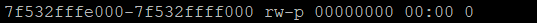
\includegraphics{3_1_2_all.png}


\begin{question}
Βρείτε και τυπώστε τη φυσική διεύθυνση μνήμης στην οποία απεικονίζεται η εικονική 
διεύθυνση του buffer (τη διεύθυνση όπου βρίσκεται αποθηκευμένος στη
φυσική κύρια μνήμη). Τι παρατηρείτε και γιατί;
\end{question}

\begin{codeless}{c}
/*
	 * Step 3: Find the physical address of the first page of your buffer
	 * in main memory. What do you see?
	 */

	printf(RED "\nStep 3: Find and print the physical address of the "
		"buffer in main memory. What do you see?\n" RESET);
	press_enter();

	/*
	 * TODO: Write your code here to complete Step 3.
	 */

	pa = get_physical_address((uint64_t)heap_private_buf);
	printf("This is the physical address of the buffer: %ld", pa);
\end{codeless}

Όταν προσπαθούμε να τυπώσουμε τη φυσική διεύθυνση μνήμης, παρατηρούμε ότι η εικονική 
διεύθυνση 0x7f61405cb0000 δεν είναι αντιστοιχισμένη και δεν έχει κατανεμηθεί φυσική 
μνήμη. 
Αυτό συμβαίνει επειδή το λειτουργικό σύστημα χρησιμοποιεί την τεχνική της 
'Σελιδοποίησης κατ' απαίτηση'. 
Αυτή η τεχνική σημαίνει ότι οι σελίδες μνήμης φορτώνονται στη φυσική μνήμη μόνο όταν 
υπάρχει αναφορά σε αυτές με δεδομένα. 
Με άλλα λόγια, μόνο όταν προσπαθήσουμε να προσπελάσουμε τη συγκεκριμένη μνήμη, τότε 
τα δεδομένα θα μεταφερθούν στη φυσική μνήμη.

\centerline{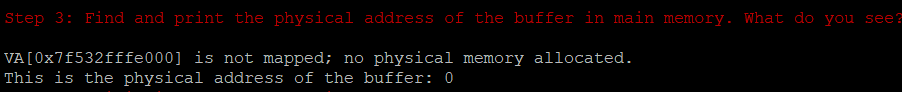
\includegraphics[width=1\textwidth]{3_1_3.png}}

\begin{question}
Γεμίστε με μηδενικά τον buffer και επαναλάβετε το \textbf{Βήμα 3}. Ποια αλλαγή 
παρατηρείτε;
\end{question}

\begin{codeless}{c}
    /*
	 * Step 4: Write zeros to the buffer and repeat Step 3.
	 */

	printf(RED "\nStep 4: Initialize your buffer with zeros and repeat "
		"Step 3. What happened?\n" RESET);
	press_enter();

	/*
	 * TODO: Write your code here to complete Step 4.
	 */

	memset(heap_private_buf, 0, buffer_size);

	pa = get_physical_address((uint64_t)heap_private_buf);
	
	printf("This is the physical address of the buffer: %ld", pa);
\end{codeless}

Παρατηρούμε ότι μας επιστρέφεται η φυσική διεύθυνση μνήμης στην οποία απεικονίζεται 
η εικονική διεύθυνση του buffer. Αυτό γίνεται διότι αυτή τη φορά σε αντίθεση με την 
προηγούμενη έχουμε προσθέσει δεδομένα στον buffer και όπως αναφέραμε παραπάνω λόγο της 
τεχνικής Demand Paging αυτή τη φορά γίνεται αναφορά στη μνήμη.

\centerline{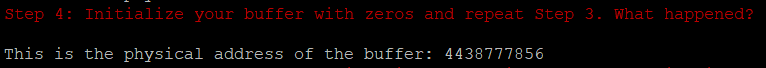
\includegraphics{3_1_4.png}}

\begin{question}
Χρησιμοποιείστε την \textbf{mmap()} για να απεικονίσετε (memory map) το αρχείο 
\textbf{file.txt} στον χώρο διευθύνσεων της διεργασίας σας και να τυπώσετε το 
περιεχόμενό του. Εντοπίστε τη νέα απεικόνιση (mapping) στον χάρτη μνήμης.
\end{question}

\begin{codeless}{c}
    /*
	 * Step 5: Use mmap(2) to map file.txt (memory-mapped files) and print
	 * its content. Use file_shared_buf.
	 */
	printf(RED "\nStep 5: Use mmap(2) to read and print file.txt. Print "
		"the new mapping information that has been created.\n" RESET);
	press_enter();
	/*
	 * TODO: Write your code here to complete Step 5.
	 */
	
	if(fstat(fop, &sb) == -1)
	{
		perror("couldn't get file size.\n");
	}
	
	printf("File size is %ld\n",sb.st_size);

	file_shared_buf = mmap(NULL, sb.st_size, PROT_READ | PROT_WRITE, MAP_PRIVATE, fop, 0);
	
	printf("Printing characters one by one next \n");	
	
	for (int i=0; i < sb.st_size; i++)
	{	
		printf("%c", file_shared_buf[i]);
	}
	
	printf("\n");

	show_maps();
\end{codeless}

\centerline{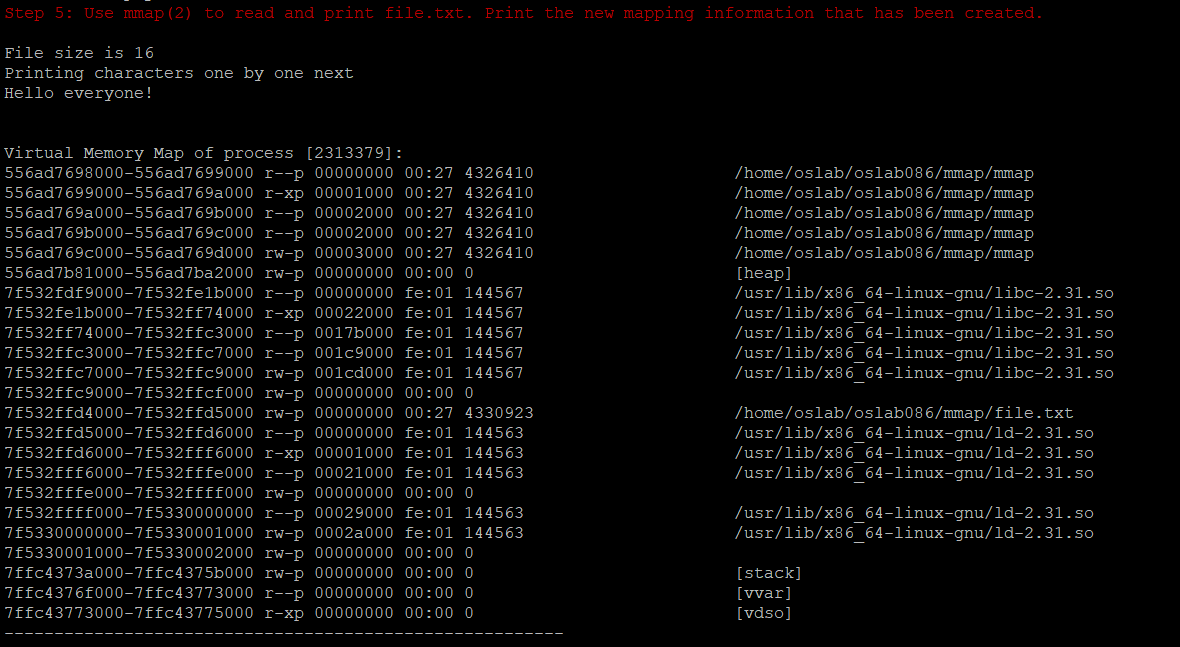
\includegraphics[width=1\textwidth]{3_1_5.png}}

Η νέα απεικόνιση βρίσκεται στη γραμμή :

\centerline{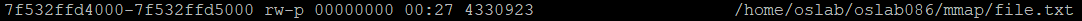
\includegraphics[width=1\textwidth]{3_1_5_new.png}}

Αυτό υποδεικνύει ότι η περιοχή μνήμης από 7f532ffd4000 έως 7f532ffd5000
έχει χαρτογραφηθεί στο αρχείο “file.txt”. 
Η περιοχή αυτή έχει δικαιώματα ανάγνωσης (r--p), αλλά όχι εγγραφής ή εκτέλεσης.

\begin{question}
Χρησιμοποιείστε την \textbf{mmap()} για να δεσμεύσετε έναν νέο buffer, διαμοιραζόμενο
(shared) αυτή τη φορά μεταξύ διεργασιών με μέγεθος μιας σελίδας. Εντοπίστε τη
νέα απεικόνιση (mapping) στο χάρτη μνήμης.
\end{question}

\begin{codeless}{c}
    /*
    * Step 6: Use mmap(2) to allocate a shared buffer of 1 page. Use
    * heap_shared_buf.
    */

   printf(RED "\nStep 6: Use mmap(2) to allocate a shared buffer of size "
       "equal to 1 page. Initialize the buffer and print the new "
       "mapping information that has been created.\n" RESET);
   press_enter();

   /*
    * TODO: Write your code here to complete Step 6.
    */
   
   heap_shared_buf = mmap(NULL, buffer_size, PROT_READ | PROT_WRITE, MAP_SHARED | MAP_ANONYMOUS, -1, 0);

   printf("Allocated memory at %p\n", heap_shared_buf);

   show_maps();
\end{codeless}

\centerline{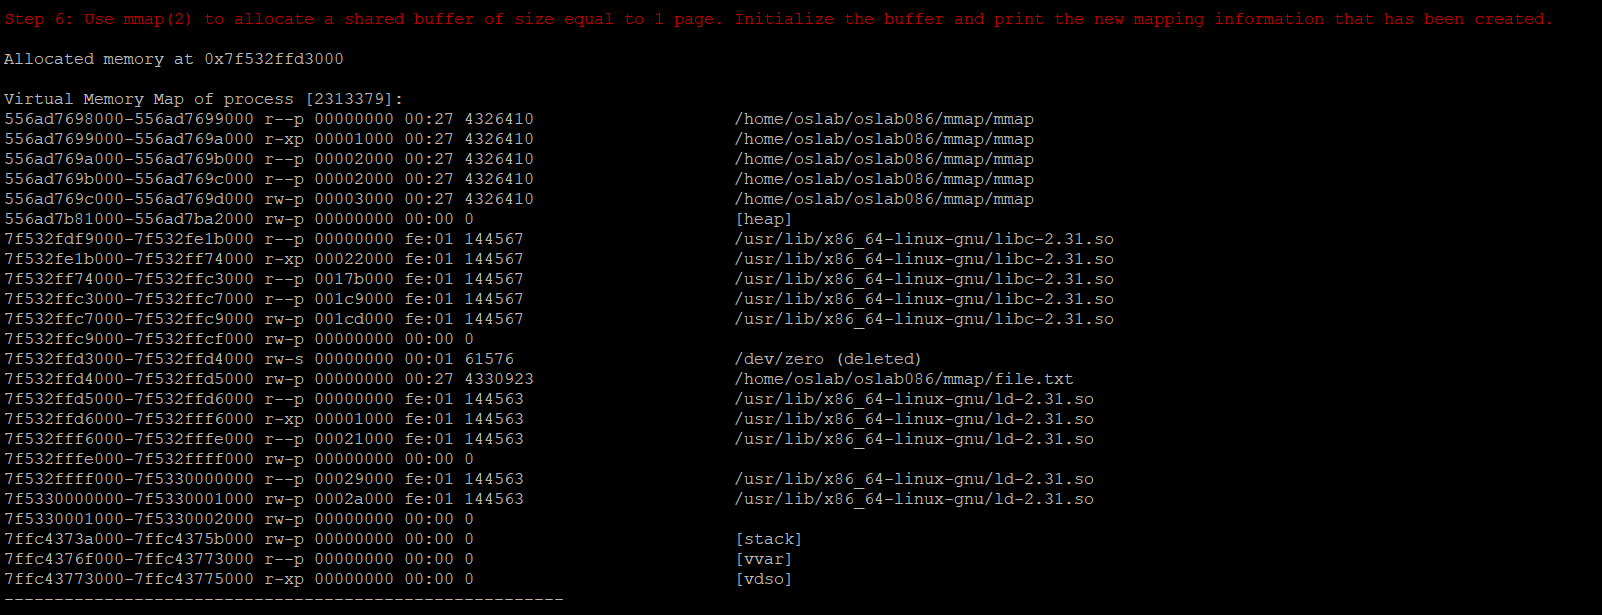
\includegraphics[width=1\textwidth]{3_1_6.png}}

Στον χάρτη μνήμης, η νέα απεικόνιση φαίνεται στη γραμμή:

\centerline{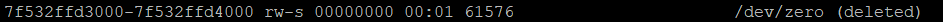
\includegraphics[width=1\textwidth]{3_1_6_ShB.png}}

Αυτό υποδεικνύει ότι η περιοχή μνήμης από 0x7f61405a0000 έως 0x7f61405a1000 έχει χαρτογραφηθεί. 
Η περιοχή αυτή έχει δικαιώματα ανάγνωσης και εγγραφής (rw-s), και χρησιμοποιείται για διαμοιραζόμενη μνήμη.

Στο σημείο αυτό καλείται η συνάρτηση \textbf{fork()} και δημιουργείται μια νέα διεργασία.

\begin{codeless}{c}
	p = fork();
	
	if (p < 0)
	{
		die("fork");
	}
	if (p == 0) 
	{
		child();
		return 0;
	}

	parent(p);
\end{codeless}

\begin{question}
Τυπώστε τους χάρτες της εικονικής μνήμης της γονικής διεργασίας και της 
διεργασίας παιδιού. Τι παρατηρείτε?
\end{question}

Στην διεργασία παιδί:

\begin{codeless}{c}
    /*
    * Step 7 - Child
    */
   
   if (0 != raise(SIGSTOP)) 
   {
       die("raise(SIGSTOP)");
   }
   
   /*
    * TODO: Write your code here to complete child's part of Step 7.
    */
   
   show_maps();
\end{codeless}

Στην γονική διεργασία:

\begin{codeless}{c}
    /* Wait for the child to raise its first SIGSTOP. */
	if (-1 == waitpid(child_pid, &status, WUNTRACED))
		die("waitpid");

	/*
	 * Step 7: Print parent's and child's maps. What do you see?
	 * Step 7 - Parent
	 */
	
	printf(RED "\nStep 7: Print parent's and child's map.\n" RESET);
	press_enter();

	/*
	 * TODO: Write your code here to complete parent's part of Step 7.
	 */
	
	show_maps();
	
	if (-1 == kill(child_pid, SIGCONT))
	{
		die("kill");
	}
	if (-1 == waitpid(child_pid, &status, WUNTRACED))
	{
		die("waitpid");
	}
\end{codeless}

\centerline{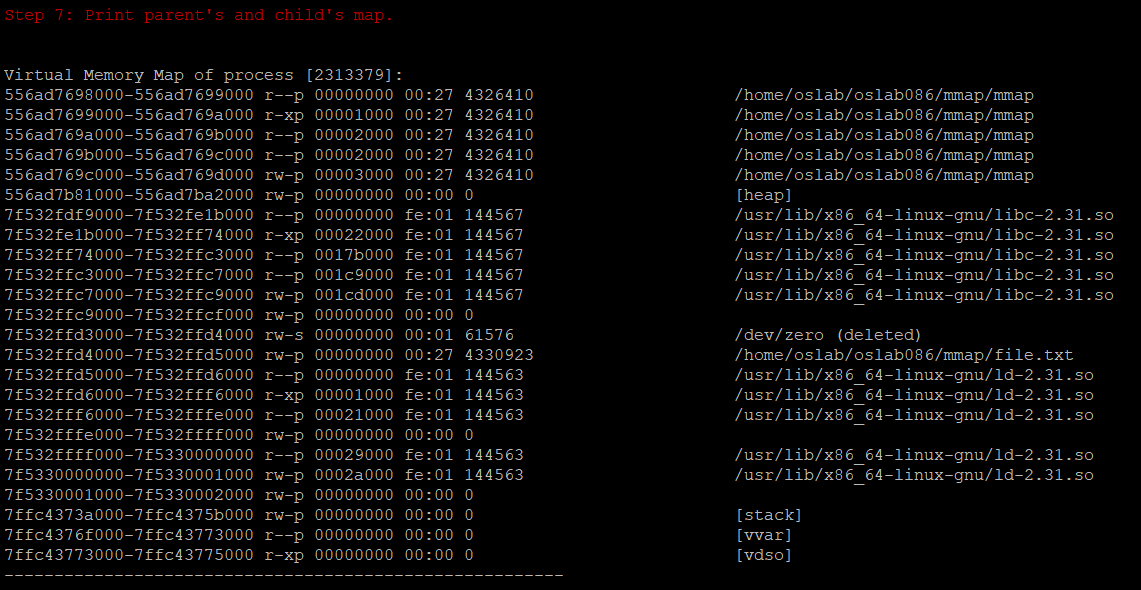
\includegraphics[width=1\textwidth]{3_1_7.png}}
\centerline{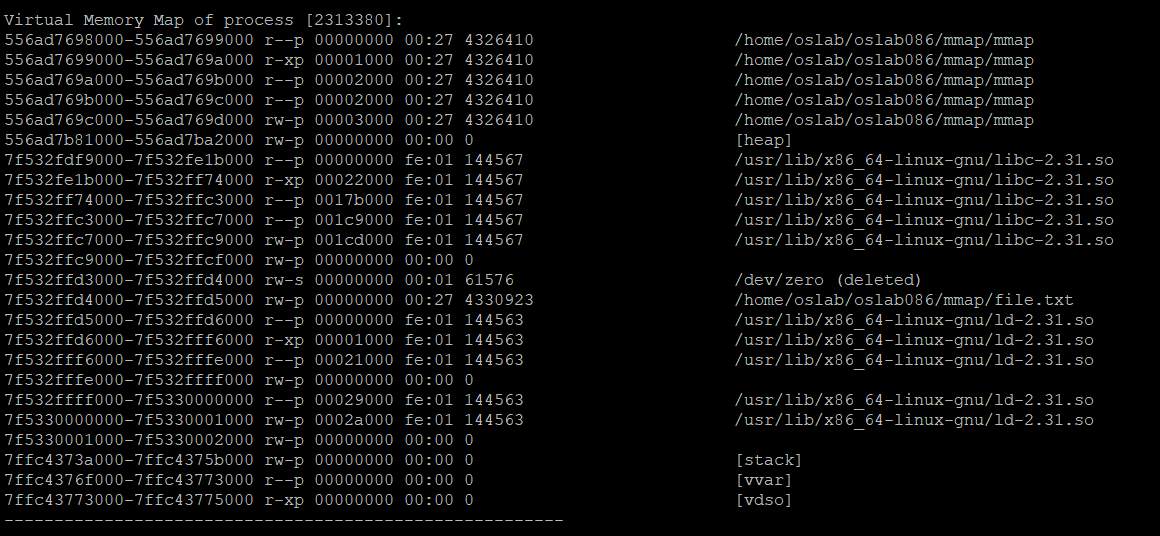
\includegraphics[width=1\textwidth]{3_1_7b.png}}

Παρατηρούμε ότι οι χάρτες μνήμης της γονικής και της παιδικής διεργασίας είναι σχεδόν 
ταυτόσημοι. 
Οι χάρτες μνήμης της γονικής και της παιδικής διεργασίας είναι σχεδόν ταυτόσημοι. 
Οι περιοχές που δημιουργήθηκαν με mmap() και χρησιμοποιούν το /dev/zero ως 
κοινόχρηστη μνήμη (shared memory) εμφανίζονται και στους δύο χάρτες μνήμης. 
Αυτό δείχνει ότι η κοινόχρηστη μνήμη είναι πραγματικά κοινόχρηστη μεταξύ 
των διεργασιών. 
Οι προστασίες μνήμης (όπως r-xp, rw-p, r--p) παραμένουν οι ίδιες τόσο για τη 
γονική όσο και για την παιδική διεργασία, διασφαλίζοντας ότι οι άδειες 
πρόσβασης διατηρούνται κατά την αντιγραφή του χώρου διευθύνσεων.

\pagebreak

\begin{question}
Βρείτε και τυπώστε τη φυσική διεύθυνση στη κύρια μνήμη του private buffer (Βήμα
3) για τις διεργασίες γονέα και παιδιού. Τι συμβαίνει αμέσως μετά το \textbf{fork}?
\end{question}

Στην διεργασία παιδί:

\begin{codeless}{c}
    /*
    * Step 8 - Child
    */
   
   if (0 != raise(SIGSTOP))
   {
       die("raise(SIGSTOP)");
   }
   
   /*
    * TODO: Write your code here to complete child's part of Step 8.
    */
   
   pa = get_physical_address((uint64_t)heap_private_buf);
   
   printf("This is the physical address of the child: %ld\n", pa);
\end{codeless}

Στην γονική διεργασία:

\begin{codeless}{c}
    /*
    * Step 8: Get the physical memory address for heap_private_buf.
    * Step 8 - Parent
    */
   
   printf(RED "\nStep 8: Find the physical address of the private heap "
       "buffer (main) for both the parent and the child.\n" RESET);
   press_enter();

   /*
    * TODO: Write your code here to complete parent's part of Step 8.
    */
   
   pa = get_physical_address((uint64_t)heap_private_buf);
       
   printf("This is the physical address of the parent: %ld\n", pa);

   if (-1 == kill(child_pid, SIGCONT))
   {
       die("kill");
   }
   if (-1 == waitpid(child_pid, &status, WUNTRACED))
   {
       die("waitpid");
   }

\end{codeless}

Όπως φαίνεται και στην εικόνα:

\centerline{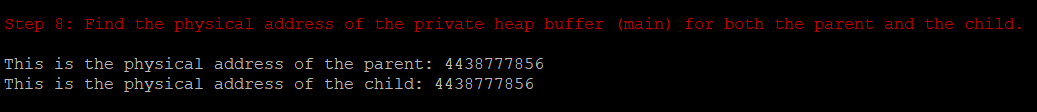
\includegraphics[width=1\textwidth]{3_1_8.png}}

Μετά την fork() οι διευθύνσεις είναι ίδιες. Ο λόγος είναι η τεχνική Copy On Write (COW), 
κατά την οποία το λειτουργικό δεν αντιγράφει κατευθείαν όλη τη μνήμη του γονέα στο παιδί. 
Αντ' αυτού, η πραγματική αντιγραφή της σελίδας συμβαίνει μόνο αν κάποια από τις 
διεργασίες (γονέας ή παιδί) προσπαθήσει να γράψει σε αυτήν τη σελίδα. 
Τότε, δημιουργείται ένα αντίγραφο της σελίδας και οι δύο διεργασίες πλέον έχουν 
τη δική τους έκδοση της σελίδας στη μνήμη. 
Αυτή η τεχνική βελτιώνει την απόδοση και εξοικονομεί μνήμη, καθώς οι σελίδες μνήμης 
δεν αντιγράφονται μέχρι να χρειαστεί.

\begin{question}
Γράψτε στον private buffer από τη διεργασία παιδί και επαναλάβετε το \textbf{Βήμα 8}. 
Τι αλλάζει και γιατί?
\end{question}

Στην διεργασία παιδί:

\begin{codeless}{c}
    /*
    * Step 9 - Child
    */
   
   if (0 != raise(SIGSTOP))
   {
       die("raise(SIGSTOP)");
   }
   
   /*
    * TODO: Write your code here to complete child's part of Step 9.
    */
   
   memset(heap_private_buf, 0, buffer_size);
   
   pa = get_physical_address((uint64_t)heap_private_buf);
       
   printf("This is the physical address of the child %ld\n", pa);
\end{codeless}

Στην γονική διεργασία:

\begin{codeless}{c}
    /*
    * Step 9: Write to heap_private_buf. What happened?
    * Step 9 - Parent
    */
   
   printf(RED "\nStep 9: Write to the private buffer from the child and "
       "repeat step 8. What happened?\n" RESET);
   press_enter();

   /*
    * TODO: Write your code here to complete parent's part of Step 9.
    */
   
   pa = get_physical_address((uint64_t)heap_private_buf);	
   
   printf("This is the physical address of the parent: %ld\n", pa);

   if (-1 == kill(child_pid, SIGCONT))
   {
       die("kill");
   }
   if (-1 == waitpid(child_pid, &status, WUNTRACED))
   {
       die("waitpid");
   }

\end{codeless}

\centerline{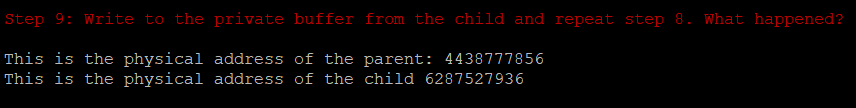
\includegraphics[width=1\textwidth]{3_1_9.png}}

Αφού γεμίσαμε τον buffer από την διεργασία παιδί και επαναλάβαμε το βήμα 8, 
παρατηρούμε ότι η φυσική διεύθυνση είναι διαφορετική για την γονική 
και παιδική διεργασία. 
Αυτό συμβαίνει γιατί, όπως αναφέραμε και στο βήμα 8, το λειτουργικό θα δημιουργήσει 
ένα ξεχωριστό αντίγραφο της σελίδας για κάθε διεργασία μόνο όταν μία από τις 
διεργασίες προσπαθήσει να γράψει στη σελίδα. 
Στην περίπτωσή μας, το κάνει η διεργασία παιδί.

\begin{question}
Γράψτε στον shared buffer (Βήμα 6) από τη διεργασία παιδί και τυπώστε τη φυσική
του διεύθυνση για τις διεργασίες γονέα και παιδιού. Τι παρατηρείτε σε σύγκριση με
τον private buffer?
\end{question}

Στην διεργασία παιδί:

\begin{codeless}{c}
    /*
    * Step 10 - Child
    */
   
   if (0 != raise(SIGSTOP))
   {
       die("raise(SIGSTOP)");
   }
   
   /*
    * TODO: Write your code here to complete child's part of Step 10.
    */
   
   *heap_shared_buf = 35;
   
   pa = get_physical_address((uint64_t)heap_shared_buf);
   
   printf("This is the physical address of the child: %ld\n", pa);
\end{codeless}

Στην γονική διεργασία:

\begin{codeless}{c}
    /*
    * Step 10: Get the physical memory address for heap_shared_buf.
    * Step 10 - Parent
    */
   
   printf(RED "\nStep 10: Write to the shared heap buffer (main) from "
       "child and get the physical address for both the parent and "
       "the child. What happened?\n" RESET);
   press_enter();

   /*
    * TODO: Write your code here to complete parent's part of Step 10.
    */

   pa = get_physical_address((uint64_t)heap_shared_buf);

   printf("This is the physical address of parent: %ld\n", pa);
   
   if (-1 == kill(child_pid, SIGCONT))
   {
       die("kill");
   }
   if (-1 == waitpid(child_pid, &status, WUNTRACED))
   {
       die("waitpid");
   }
\end{codeless}

\centerline{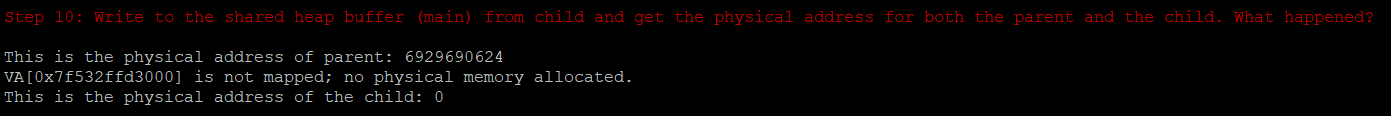
\includegraphics[width=1\textwidth]{3_1_10.png}}

Αφού γράψουμε στον κοινό buffer από τη διεργασία παιδί, παρατηρούμε ότι όταν 
προσπαθούμε να τυπώσουμε τη φυσική διεύθυνση του buffer από τις διεργασίες, 
η γονική διεργασία δεν επιστρέφει τίποτα, ενώ η παιδική διεργασία επιστρέφει 
τη φυσική διεύθυνση. 
Αυτό συμβαίνει επειδή, μετά την fork(), δεν έχουμε επιχειρήσει να γράψουμε στον 
κοινό buffer από τη γονική διεργασία. Έτσι, λόγω της τεχνικής Demand Paging, 
εφόσον δεν έχει γίνει αναφορά στον buffer, οι σελίδες του δεν έχουν μεταφερθεί 
στη φυσική μνήμη για τη γονική διεργασία.
Ο private buffer, μετά την fork(), επιστρέφει τη φυσική του διεύθυνση και από 
τις δύο διεργασίες, ακόμα κι αν δεν έχει γίνει καμία εγγραφή. 
Αυτό συμβαίνει λόγω της τεχνικής Copy-on-Write, όπου η παιδική διεργασία 
είναι αντίγραφο της γονικής μέχρι να γίνει κάποια εγγραφή. Επομένως, η φυσική 
διεύθυνση του private buffer παραμένει η ίδια για τις δύο διεργασίες μέχρι να 
συμβεί κάποια τροποποίηση.
Αντίθετα, ο shared buffer μπορεί να προσπελαστεί και από τις δύο διεργασίες, 
αλλά πρέπει πρώτα να γίνει αναφορά σε αυτόν από κάθε διεργασία ώστε οι σελίδες του 
να χαρτογραφηθούν στη φυσική μνήμη. Μόνο τότε θα μπορούν και οι δύο 
διεργασίες να τυπώσουν τη φυσική του διεύθυνση.


\begin{question}
Απαγορεύστε τις εγγραφές στον shared buffer για τη διεργασία παιδί. Εντοπίστε και
τυπώστε την απεικόνιση του shared buffer στο χάρτη μνήμης των δύο διεργασιών
για να επιβεβαιώσετε την απαγόρευση.
\end{question}

Στην διεργασία παιδί:

\begin{codeless}{c}
    /*
    * Step 11 - Child
    */

   if (0 != raise(SIGSTOP))
   {
       die("raise(SIGSTOP)");
   }

   /*
    * TODO: Write your code here to complete child's part of Step 11.
    */
   
   if(mprotect(heap_shared_buf, buffer_size, PROT_READ) == -1)
   {
       perror("mprotect");
       exit(1);
   }

   show_maps();
\end{codeless}

Ο χάρτης της παιδικής διεργασίας:

\centerline{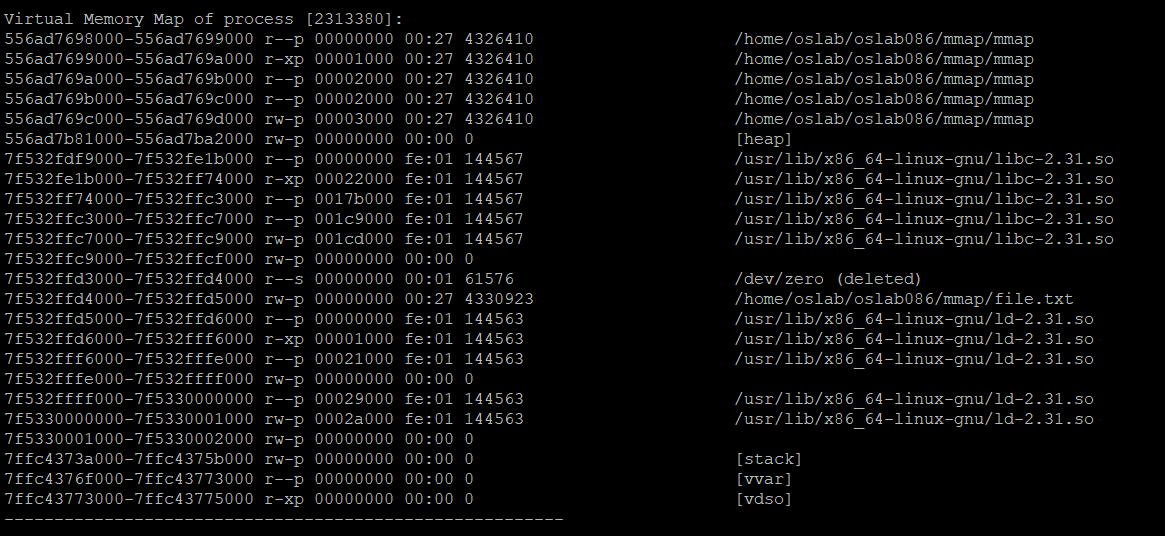
\includegraphics[width=1\textwidth]{3_1_11b.png}}

Στην γονική διεργασία:

\begin{codeless}{c}
    /*
    * Step 11: Disable writing on the shared buffer for the child
    * (hint: mprotect(2)).
    * Step 11 - Parent
    */
   
   printf(RED "\nStep 11: Disable writing on the shared buffer for the "
       "child. Verify through the maps for the parent and the "
       "child.\n" RESET);
   press_enter();

   /*
    * TODO: Write your code here to complete parent's part of Step 11.
    */
   
   show_maps();
   
   if (-1 == kill(child_pid, SIGCONT))
   {
       die("kill");
   }
   if (-1 == waitpid(child_pid, &status, 0))
   {
       die("waitpid");
   }
\end{codeless}

Ο χάρτης της γονικής διεργασίας:

\centerline{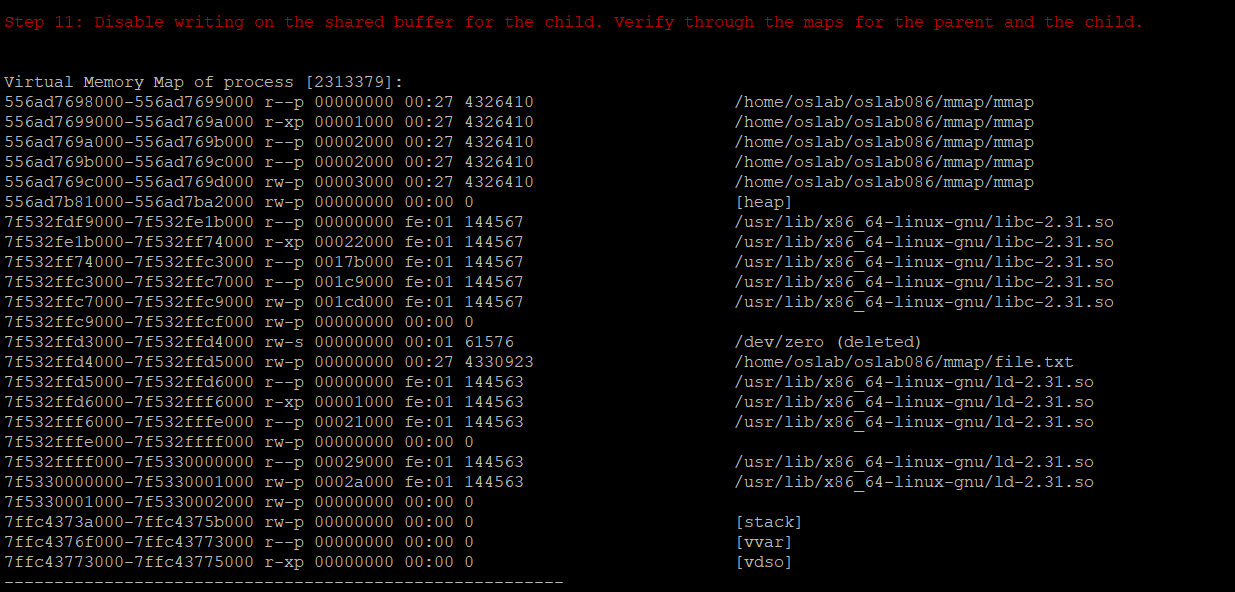
\includegraphics[width=1\textwidth]{3_1_11.png}}

Αφού απαγορεύσουμε τα δικαιώματα εγγραφής στον shared buffer από την παιδική διεργασία, 
παρατηρούμε αλλαγή στα δικαιώματα στη γραμμή που φαίνεται ο shared buffer, όπου για 
την παιδική διεργασία (r--s), ενώ για την γονική (rw-p).

Για την παιδική διεργασία:

\centerline{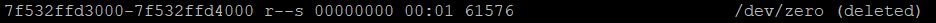
\includegraphics[width=1\textwidth]{3_1_11_ChildChange.png}}

Για την γονική διεργασία:

\centerline{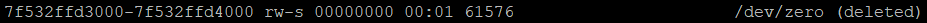
\includegraphics[width=1\textwidth]{3_1_11_Parent.png}}

\pagebreak

\begin{question}
Αποδεσμεύστε όλους τους buffers στις δύο διεργασίες.
\end{question}

Στην διεργασία παιδί:

\begin{codeless}{c}
    /*
    * Step 12 - Child
    */
   
   munmap(heap_private_buf, buffer_size);
   munmap(heap_shared_buf, buffer_size);

   /*
    * TODO: Write your code here to complete child's part of Step 12.
    */
\end{codeless}

Στην γονική διεργασία:

\begin{codeless}{c}
    /*
    * Step 12: Free all buffers for parent and child.
    * Step 12 - Parent
    */

   munmap(heap_private_buf, buffer_size);
   munmap(heap_shared_buf, buffer_size);

   /*
    * TODO: Write your code here to complete parent's part of Step 12.
    */
\end{codeless}

\pagebreak

\section{Παράλληλος υπολογισμός Mandelbrot με διεργασίες αντί για νήματα}


\subsection{Semaphores πάνω από διαμοιραζόμενη μνήμη}

\begin{question}
Ποια από τις δύο παραλληλοποιημένες υλοποιήσεις (threads vs processes) περιμένετε 
να έχει καλύτερη επίδοση και γιατί; Πώς επηρεάζει την επίδοση της υλοποίησης 
με διεργασίες το γεγονός ότι τα semaphores βρίσκονται σε διαμοιραζόμενη
μνήμη μεταξύ διεργασιών;
\end{question}

Περιμένουμε τα threads να έχουν καλύτερη επίδοση σε συγκεκριμένες περιπτώσεις, διότι
είναι ελαφρύτερα και ευκολότερα στη διαχείριση. Επιπλέον, τα threads μιας διεργασίας
μοιράζονται τον ίδιο χώρο μνήμης, πράγμα που επιτρέπει την ταχύτερη και ευκολότερη 
επικοινωνία και ανταλλαγή δεδομένων μεταξύ τους σε σύγκριση με τις διεργασίες, οι 
οποίες έχουν ξεχωριστούς χώρους μνήμης.

Το γεγονός ότι τα semaphores βρίσκονται σε διαμοιραζόμενη μνήμη μεταξύ διεργασιών 
βελτιώνει την επικοινωνία και τον συγχρονισμό τους. 
Ωστόσο, αυξάνει την πολυπλοκότητα του κώδικα και μας αφήνει ευάλωτους σε λάθη.


\subsection{Υλοποίηση χωρίς semaphores}

\begin{question}
Με ποιο τρόπο και σε ποιο σημείο επιτυγχάνεται ο συγχρονισμός σε αυτή την υλοποίηση; 
Πώς θα επηρεαζόταν το σχήμα συγχρονισμού αν ο buffer είχε διαστάσεις
NPROCS $\times$ x\_chars;
\end{question}

Ο συγχρονισμός σε αυτή την υλοποίηση επιτυγχάνεται με τη χρήση της διαμοιραζόμενης 
μνήμης για την αποθήκευση των αποτελεσμάτων της υπολογιστικής εργασίας. 
Συγκεκριμένα:
Ο buffer δημιουργείται ως κοινόχρηστη μνήμη μέσω της mmap στην 
create\_shared\_memory\_area συνάρτηση.
Κάθε διεργασία παιδί μπορεί να γράψει στον κοινόχρηστο buffer, επιτρέποντας έτσι 
την αποθήκευση των αποτελεσμάτων υπολογισμού σε ένα κοινό σημείο.
Ο buffer χρησιμοποιείται για την αποθήκευση των τιμών χρώματος κάθε γραμμής. 
Οι διεργασίες παιδί υπολογίζουν τις γραμμές του Mandelbrot set και γράφουν τα 
αποτελέσματα στον κοινόχρηστο buffer.
Εάν ο buffer είχε διαστάσεις ${NPROCS \times x\_chars}$, αυτό θα σήμαινε 
ότι κάθε διεργασία θα είχε το δικό της ξεχωριστό τμήμα του buffer. 
Σε αυτή την περίπτωση:
Κάθε διεργασία θα έγραφε στα δικά της συγκεκριμένα στοιχεία του buffer. 
Για παράδειγμα, η διεργασία i θα έγραφε στο ${buf + i * x\_chars}$.
Ο διαχωρισμός θα διασφάλιζε ότι δεν υπάρχουν συγκρούσεις, καθώς κάθε διεργασία θα 
διαχειριζόταν έναν απομονωμένο τομέα του buffer.
Η ανάγκη για πρόσθετους μηχανισμούς συγχρονισμού (π.χ., semaphores) θα ήταν μειωμένη 
ή ανύπαρκτη, διότι κάθε διεργασία θα είχε αποκλειστική πρόσβαση στα δικά της δεδομένα.

\end{document}
